
\lecture{Introduction}{Introduction}
\section{Introduction}

\title{Statistics}
\subtitle{Introduction To Statistics and Course Information}

%\author{Kelly Black}
%\institute{Clarkson University}
\date{25 August 2014}

\begin{frame}
  \titlepage
\end{frame}

%\begin{frame}
%  \frametitle{Outline}
%  \tableofcontents[hideothersubsections,sectionstyle=show/hide]
%\end{frame}


\subsection{Class Information}


\begin{frame}
  \frametitle{Class Information}

\begin{description}
\item[Textbook] {\em Probability and Statistics for Engineers and
    Scientists}, Fourth Edition, by Anthony Hayter,
  Brooks/Cole;. (ISBN 9781111827045) The book is available at the
  bookstore as well as many on-line outlets.

\end{description}

\end{frame}


\begin{frame}
  \frametitle{Class Information}

\begin{description}
\item[Grading] %~ \\ %\samepage
  
  The final grades are calculated using the following distribution:
    \begin{tabular}[t]{rl}
      55\% & Three Exams. \\
      15\% & Quizzes. \\
      15\% & Webworks. \\
      10\% & Reports. \\
      5\%  & Clickers
    \end{tabular}

  
    At the end of the semester we assign letter grades as follows:
    97\% for an A+, 93\% for an A, 90\% for an A-, 
    87\% for a  B+, 83\% for an B, 80\% for a B-, 
    77\% for a  C+, 73\% for an C, 70\% for a C-, 
    and \%60 for a D.

\end{description}

\end{frame}



\begin{frame}
  \frametitle{Class Information}

\begin{description}
\item[Exam Dates] The first test is tentatively scheduled for 2
  October from 7:00pm to 8:15pm. The second test is tentatively
  scheduled for 12 November from 8:30pm to 9:45pm. The rooms will be
  announced in class. The third test will take place during finals
  week.  You should bring your own pencils, blank paper, calculators,
  and good luck charms.  The professor will not have any spare
  materials.
 
\end{description}

\end{frame}

\begin{frame}
  \frametitle{Class Information}

\begin{description}
\item[Quiz] There will be a quiz every other week in class. The
  quizzes will be similar to the posted homework problems. The lowest
  quiz score will be dropped.
\end{description}

\end{frame}


\begin{frame}
  \frametitle{Class Information}

\begin{description}
  \item[Clickers] A portion of your grade is for classroom attendance
    and participation. This is measured using clickers. Each day one
    or more questions will be asked, and you will be asked to respond
    using the clicker. The clicker that we are using is from Turning
    Point Technologies, and we recommend that you use the ResponseCard
    RF LCD clicker. You can purchase the clicker at
    \url{https://store.turningtechnologies.com} The Clarkson
    University promotional code is Z0k0.

\end{description}

\end{frame}

\begin{frame}
  \frametitle{Clickers}

  We will start using the clickers this Friday. Each day one or more
  questions will be asked.

  You need to register your clicker. Go to our course page on moodle:
  \begin{enumerate}
  \item Choose the ``clicker ID'' option at the top of the page.
  \item Enter your clicker Device ID (found on the back of the
    clicker.)
  \item Click on the submit button.
  \item Click on the ``next'' button.
  \item Click on ``Submit all and finish.''
  \item Confirm your choice.
  \item Click on ``Finish Review'' at the bottom of the page.
  \end{enumerate}

  If you do not click on ``Finish Review'' your device ID may not be saved.

  Note: Zero is not an ``O''  !!!
  
\end{frame}


\begin{frame}
  \frametitle{Class Information}

\begin{description}
  \item[Webwork] Webwork is a web based homework system. You can find
    it at the following URL: \\
    \url{http://black.sc.clarkson.edu/webwork2/}.
\end{description}

\end{frame}


\begin{frame}
  \frametitle{Class Information}

\begin{description}
  \item[Academic Accommodations] If you require any kind of special
    accommodation please come see me.  Requests for academic
    accommodations must be made during the first three weeks of the
    semester, except for unusual circumstances.  Students must
    register with the Office of Accommodative Services, located in the
    Student Success Center, 110 ERC, to verify their eligibility for
    appropriate accommodations.


\end{description}


\end{frame}


\begin{frame}{Important Terms}

  \begin{description}
  \item[Event:] Something that \textit{can} happen.
  \item[Outcome:] Something that did happen.
  \item[Experiment:] A structured activity that includes the
    measurement of the outcomes of the activity after predefined and
    intentional changes to some aspect of the events.
  \item[Observational Study:] A structured activity that includes the
    measurement of the outcomes of the activity without intentional
    changes to the events.
  \item[Expected Outcome:] The ``average'' of the possible outcomes.
  \item[Variation:] Some measure of the spread of possible outcomes.
  \end{description}
  
\end{frame}

\begin{frame}{Probability vs. Statistics}

  ``Probability'' is an idealized notion. If we repeat the experiment
  an infinite number of times we ask what do we \textit{expect will} happen.

  \vfill

  ``Statistics'' is the study of how to interpret data. We ask what
  ``did'' happen and what does it imply about the underlying
  probabilities?

  \vfill

  \uncover<2->%
  {

    Problem: We need to have a basic understanding of probability
    before we can do statistics.

  }
  
\end{frame}

\begin{frame}{Expectations}
\vspace*{-2em}
  Our evaluation is based on the following expectations: \\
\footnotesize \hspace*{-2em}
\begin{tabular}{|l@{\hspace{2em}}l|} \hline
  Quality of Work    & Expectations \\ \hline
  Needs Improvement  & Cannot use more than one principle to solve a problem. \\
                     & Cannot identify and categorize the question
                       being asked. \\ \hline
  Satisfactory       & Know basic formulas and distributions by name. \\
                     & Can use multiple rules and ideas to solve a
                       given problem.\\ 
                     & Can recognize and categorize questions. \\
 \hline
  Good               &  Can identify relationships between different
                        basic formulas. \\
                     &  Can identify the connections between ideas in
                        different topics. \\ \hline
  Excellent          &  Can derive new relationships constructed from
                        basic formulas. \\
                     &  Can use ideas from different topics to create
                        new decision \\
                     & making approaches. \\ \hline
\end{tabular}
\end{frame}

\begin{frame}{Relationships Between Topics}
  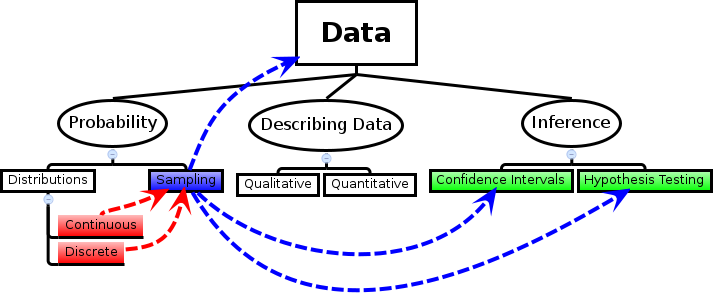
\includegraphics[height=4cm]{bigIdeas}
\end{frame}

\begin{frame}{Experiment}

  We perform an experiment, gather data, calculate the statistics, and
  then make decisions. 

  \vfill

  \uncover<2>{
    
    \redText{No!} We make a lot of decisions throughout. This is all one
    experiment. All aspects are part of the experiment and must be
    considered \textbf{\sc before} you do anything else.

  }

  \vfill
  
\end{frame}



\begin{frame}{Definitions}

  \begin{description}
  \item[Event:] Something that \textit{can} happen.
  \item[Outcome:] Something that did happen.
  \item[Experiment:] A structured activity that includes the
    measurement of the outcomes of the activity after predefined and
    intentional changes to some aspect of the events.
  \item[Observational Study:] A structured activity that includes the
    measurement of the outcomes of the activity without intentional
    changes to the events.
  \item[Expected Outcome:] The ``average'' of the possible outcomes.
  \item[Variation:] Some measure of the spread of possible outcomes.
  \end{description}
  
\end{frame}


\begin{frame}{Probability}

  \begin{definition}[Probability]
    ``\textbf{Probability} is the measure of the likelihood of a random
    phenomena or chance behavior. Probability describes the long-term
    proportion with which a certain \textbf{outcome} will occur in
    situations with short-term uncertainty.'' 
  \end{definition}

  
\end{frame}



\begin{frame}{Caveats}

  ``Probability'' is an idealized notion. If we repeat the experiment
  an infinite number of times we ask what \textit{will} happen.

  \vfill

  ``Statistics'' is the study of how to interpret data. We ask what
  ``did'' happen and what does it imply about the underlying
  probabilities?

  \vfill

\end{frame}


\begin{frame}{Sample Space}

  \begin{definition}[Sample Space]
    The sample space is the set of all possible outcomes.
  \end{definition}

  
\end{frame}


% LocalWords:  Clarkson pausesection hideallsubsections Cuby Webworks Webwork
% LocalWords:  ResponseCard Fukushima hideothersubsections sectionstyle

